% File project.tex
%% Style files for ACL 2021
\documentclass[11pt,a4paper]{article}
\usepackage[hyperref]{acl2021}
\usepackage{times}
\usepackage{booktabs}
\usepackage{todonotes}
\usepackage{latexsym}
\renewcommand{\UrlFont}{\ttfamily\small}

% This is not strictly necessary, and may be commented out,
% but it will improve the layout of the manuscript,
% and will typically save some space.
\usepackage{microtype}

\aclfinalcopy 

\newcommand\BibTeX{B\textsc{ib}\TeX}

\title{11-777 Report 1: Dataset Proposal and Analysis}

\author{
  Shashwat Chawla\thanks{\hspace{4pt}Everyone Contributed Equally} \hspace{2em} Yatharth Ahuja$^*$ \hspace{2em} Pujith Kachana$^*$ \hspace{2em} Ming-Feng Li$^*$ \\
  \texttt{\{shashwac, yahuja, pkachana, mingfenl\}@andrew.cmu.edu}
  }

\date{}

\begin{document}
\maketitle

\section{Problem Definition and Dataset Choice (1 page)}
% A dense map of the environment
Accurate 3D localization is essential for autonomous robotic systems to precisely track the movement of autonomous driving cars, robots, or drones. By integrating RGB or LiDAR sensors, estimated camera poses from 3D localization can further facilitate the dense map reconstruction of 3D scenes. Visual Simultaneous Localization and Mapping (SLAM) is becoming increasingly important due to the widespread availability of cameras and the rich information provided by images. Visual odometry (VO), a key component of visual SLAM, has seen notable progress through geometry-based methods \cite{lsd-slam}, \cite{orb-slam}, \cite{spa-odom}. However, these methods are often unreliable in challenging conditions such as varying illumination, dynamic environments, and rapid movements. Deep neural network-based methods have demonstrated the ability to learn more robust feature extractors than traditional, engineered ones, leading to more capable VO models \cite{vo-dnn}, \cite{sfm-net}. 

One such method, TartanVO \cite{tartanvo2020corl}, has shown impressive real-world performance, even when trained solely on simulated data. This is attributed to the use of diverse scenes during training, an up-to-scale loss function to address scale ambiguity, and an intrinsic layer that supports generalization across different cameras. This project aims to enhance TartanVO (which currently works on image pairs) by fusing LiDAR data with camera images. The model will be trained using the TartanAir dataset and evaluated on real-world datasets like KITTI and EuROC to assess its real-world applicability. The project will be co-supervised by Professor Wenshen Wang.


\subsection{What phenomena or task does this dataset help address?}
%Essentialy we target to estimate the odometry of the ego agent, which helps us know how the agent traverses in the space.%
Reasoning about an agents ego-motion during autonomous operations is crucial as it helps the agent understand the scene and plan for downstream tasks more accurately. %The TartanVO project attempted to learn the odometry estimation using only the monocular input which is fundamentally insufficient for understanding the scale of estimations. Thus, we hope the complementary LiDAR data can help refine the estimations.%
The TartanAir dataset offers large-scale synthetic data for various vision tasks to allow for precise, multi-modal learning, specifically for the purpose of navigation. The dataset contains RGB, depth, LiDAR, flow, segmentation, and odometry data for multiples cameras through a diverse set of scenes and trajectories, enabling a large set of modality combinations to be explored for various visual navigation tasks.

\subsection{What about this task is fundamentally multimodal?}
Visual odometry is a complex task that requires a precise understanding of the relative ego-motion and object dynamics. Currently, there is no single modality that can effectively capture enough data to enable this reasoning. Monocular images lack the necessary depth information to understand scale, while depth and LiDAR data are often very noisy and do not have salient enough features to compute correspondences between frames. Given that there is no satisfactory unimodal solution, we propose that visual odometry should therefore be seen as a fundamentally multimodal task. Monocular RGB input will help us get rich visual features in the contextual scene, whereas the LiDAR modality will help us consider and construct semantic sense in the same. We can expect some overlap in the information between these modalities due to possible correlations between features and their depth - but they also complement each other by providing separate information.

\subsection{Hypothesis}
Due to the limitations of sensor data in real-world cases, only RDB images and LiDAR (or sparse depth map) data are available, we majorly implement a multi-modal model that takes RGB and LiDAR data as input. However, we expect that the fusion of various data from different modalities like segmentation, optical flow, and dense depth map could effectively benefit our model in learning more general scene understandings in the model training stage.

We believe there are several cross-modal information that can be used to improve the model performance:
  \begin{enumerate}
    \item A major shortcoming of monocular RGB data for odometry is its lack of depth information. \cite{tartanvo2020corl} circumvents this problem by using a scale-invariant loss, thereby recovering a motion vector between two frames as opposed to an absolute pose. We believe the addition of rich, inherently 3D data for LiDAR will alleviate this issue.
    
    \item A large problem with LiDAR data for odometry is the sparsity and weak features. Classical approaches use algorithms such as Iteractive Closest Point (ICP) to estimate correspondences and poses between frames; however, this is a slow and noisy process. We believe the addition of strong visual features from RGB data will help address this issue.
    
    \item To fully exploit cross-modal data, including segmentation, optical flow, and dense depth maps in our training datasets, we propose pre-training the model backbone to simultaneously predict multiple modalities. This approach enables the model to learn an encoder that could extract more comprehensive semantic and spatial information. Specifically, we design a shared encoder that processes both RGB images and LiDAR points as input, while separate decoders are used for each modality to predict their respective outputs.
    
  \end{enumerate}
\subsection{Expertise}
We have the following expertise in the underlying modalities required by this task:
  \begin{enumerate}
      \item Shashwat Chawla: Prior industrial experience in Visual SLAM, perception, and state-estimation. Experience working with differential-drive mobile robots, manipulators, and drones.   
      \item Yatharth Ahuja: Prior experience in perception and controls for robots. Have taken courses in Visual Learning, Robot Autonomy in Spring 2024. Publications in Visual SLAM and Learning based methods.
      \item Pujith Kachana: Research experience in 3D learning, 3D reconstruction, and 2D-3D fusion. Experience working with TartanAir dataset and learning-based odometry.
      \item Ming-Feng Li: Research experience in 3D vision, including 3D generation using pre-trained diffusion models, object 6D pose estimation, and 3D reconstruction.
  \end{enumerate}

% \clearpage

\section{Dataset Analysis (1 page)}
\subsection{Dataset properties}
The TartanAir dataset is a large-scale, synthetically generated vision and navigation dataset rendered using the Unreal Engine. The synthetic nature of the data guarantees precise, dense measurements, while the well-developed rendering process keeps the data reasonably photo-realistic. There are currently two versions of the TartanAir, and a larger TartanAir v2 that is still unreleased. We report the statistics for TartanAir below as they have been released, but hope to use TartanAir v2 to actually train our models. A few known TartanAir v2 statistics are also reported. \\

Data Statistics: 
 TartanAir
 \begin{enumerate}
     \item Data size: 4TB 
     \item Environments: 30 diverse environments containing indoor and outdoor scenes
     \item Sequences: 1037 long drone motion sequences
     \item Frames: Over 1 million frames, around 500-4000 frames per sequence
     \item Data Modalities: RGB, LiDAR, Depth
% Stereo RGB, Flow, Segmentation, Occupancy Map, Camera Poses, Trajectory
    \item Rig: 2 pinhole camaras

 \end{enumerate}
 TartanAir v2
  \begin{enumerate}
     \item Data size: 40TB 
     \item Environments: 100 diverse environments containing indoor and outdoor scenes
     \item Data Modalities: RGB, LiDAR, Depth
     % , Stereo RGB, Flow, Segmentation, Occupancy Map, Camera Poses, Trajectory
    \item Rig: 6 pinhole camaras, 1 fisheye camera, 1 equirectangular camera
 \end{enumerate}


\subsection{Compute Requirements}
  \begin{enumerate}
    \item Atleast one GPU with 16GB VRAM and 4TB disk space
    \item AWS credits from class, and Computing Cluster with access to TartanAir dataset
    
  \end{enumerate}

\begin{figure}[h]
\centering
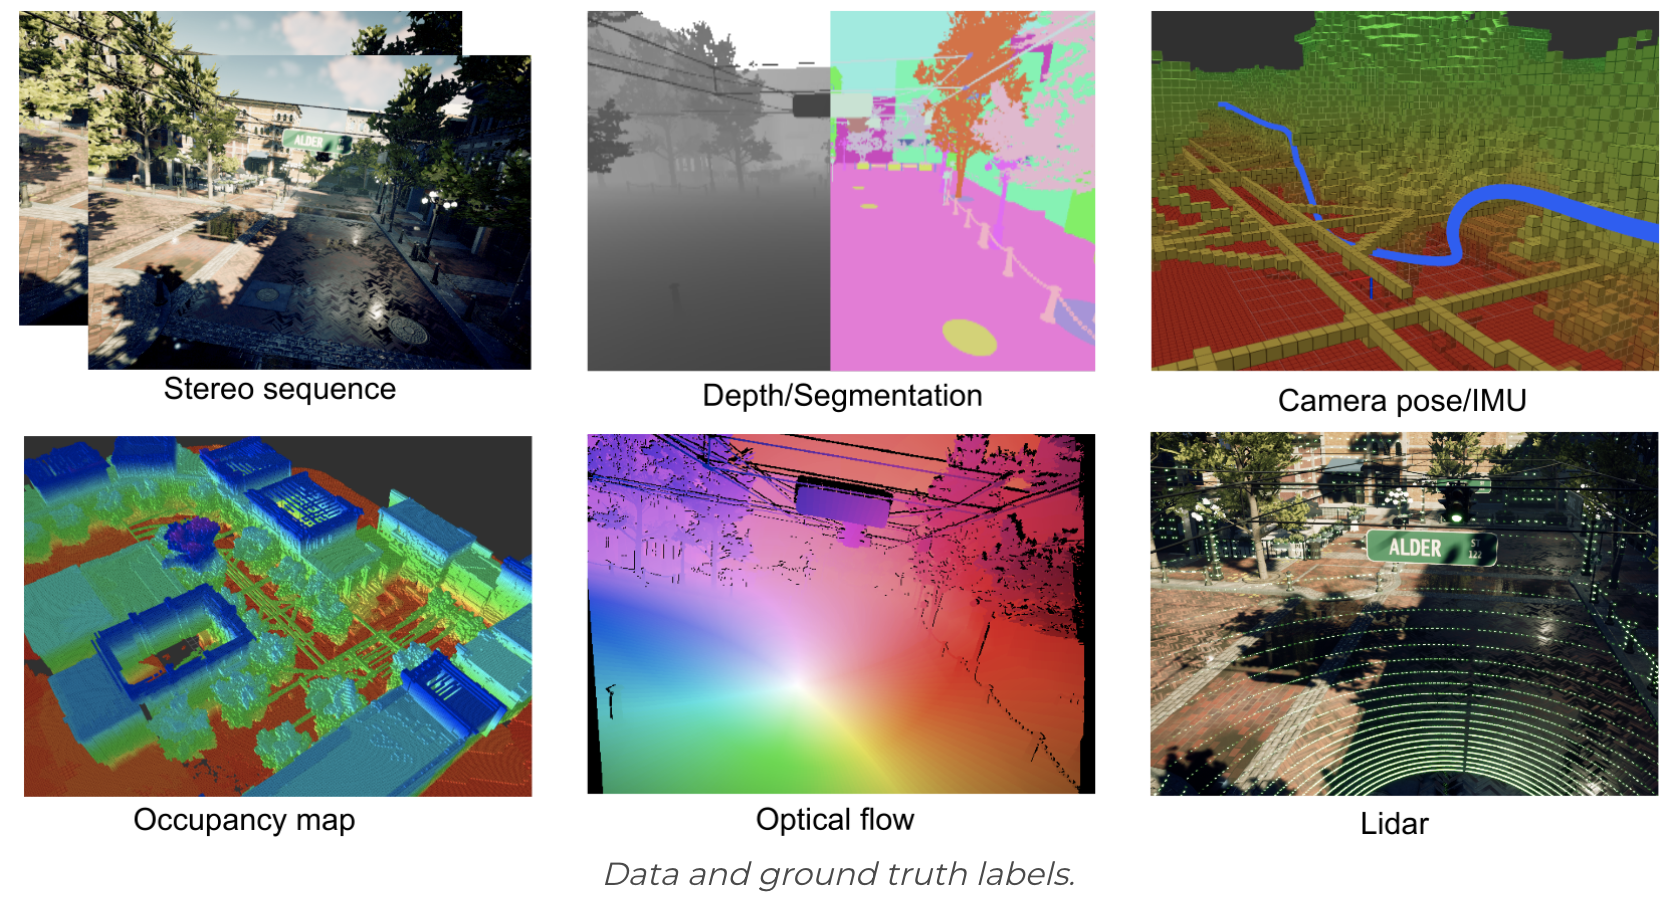
\includegraphics[width=\linewidth]{Figure/dataset_samples.png}
\caption{
    Data of different modalities in the dataset.
}
\label{fig:dataset-samples}
\end{figure}


\subsection{Modality analysis}
  \begin{enumerate}
    % \item Lexical diversity, sentence length, ...
    % \item Average number of objects detected per image
    % \item Degrees of freedom, number of articulated objects,
    % ...
    \item RGB: This modality presents feature rich data which can be exploited to understand and contrast the views in the context. However, monocular RGB data for odometry lacks of depth information, where it can take help from LiDAR inputs. 
    % \item Depth :
    \item LiDAR: Distance data helps us find semantic features and scale information. A drawback with LiDAR data for odometry is the sparsity and weak features, which can be helped with monocular input.
    % \item Optical flow:
    % \item Semantic segmentation:
    
  \end{enumerate}
  

\subsection{Metrics used}
The main metrics which we will be using to evaluate our model's performance are:

\begin{enumerate}
    \item t\_rel: Average translational RMSE drift (\%) across a fixed length.
    
    \item r\_rel: Average rotational RMSE drift (◦/100 m) across a fixed length.
\end{enumerate}

\subsection{Baselines} 
Four papers that have worked on this dataset

\textbf{TartanVO}: TartanVO is a deep learning-based VO framework designed for generalization across diverse environments and cameras, and is trained on TartanAir's RGB, flow, and pose data. It uses optical-flow prediction as an intermediate task to predict up-to-scale pose estimation. It outperforms traditional and learning-based VO methods in unseen, challenging environments.\cite{tartanvo2020corl} \\

\textbf{Deep Patch VO}:  DPVO uses a novel recurrent network architecture designed for tracking image patches across time. It has been assumed that dense flow is important as it provides additional redundancy against incorrect matches. DPVO disproves this assumption, showing that it is possible to get the best accuracy and efficiency by exploiting the advantages of sparse patch-based matching over dense flow. On Standard benchmarks, DPVO outperforms all prior work, including the learning-based state-of-the-art VO system (DROID) using a third of the memory while running 3x faster on average. \cite{deepVO} \\

\textbf{DytanVO}: A supervised learning-based VO method that deals with dynamic environments. It takes two consecutive monocular frames in real-time and predicts camera ego-motion in an iterative fashion. This method achieves an average improvement of 27.7\% in ATE over state-of-the-art VO solutions in real-world dynamic environments, and performs reasonably among dynamic visual SLAM systems which optimize the trajectory on the backend. \cite{dytanvo}\\

\textbf{Salient Sparse VO}: A novel hybrid VO framework that leverages pose-only supervision, offering a balanced solution between robustness and the need for extensive labeling. The paper proposes two cost-effective and innovative designs: a self-supervised homographic pre-training for enhancing optical flow learning from pose-only labels and a random patch-based salient point detection strategy for more accurate optical flow patch extraction. These designs eliminate the need for dense optical flow labels for training and significantly improve the generalization capability of the system in diverse and challenging environments.
\cite{SuperSparse}

% \clearpage
\section{Team member contributions}
\paragraph{Shashwat Chawla} contributed to project discovery, development of the initial proposal, collaboration with Airlab, and writing sections on "Problem Definition" (Section 1) and "Baselines" (Section 2) of the paper.

\paragraph{Yatharth Ahuja} contributed towards problem description, coordinations with the TA, exploring modalities, evaluation metrics and considering some of the baselines.

\paragraph{Pujith Kachana} contributed the dataset properties, parts of the hypothesis and problem definition, and some of the baselines.

\paragraph{Ming-Feng Li} contributed towards overall discussions around the hypothesis, the approach, and dataset analysis.

% \clearpage

% Please use 
\bibliographystyle{acl_natbib}
\bibliography{references}

%\appendix



\end{document}
